\section{Introduction and general hypothesis}

\subsection{Introduction}

This report sets out the mathematical modelling of one-dimensional subcritical
and supercritical flows on which the three different hydraulic engines of the
code system \texttt{MASCARET} are based, as well as the methods of solving
equations resulting from these models.
We present below the structure of the \texttt{MASCARET} system. This report
only covers the \textit{hydraulic} part of the system.

\begin{figure}[h]
 \begin{center}
  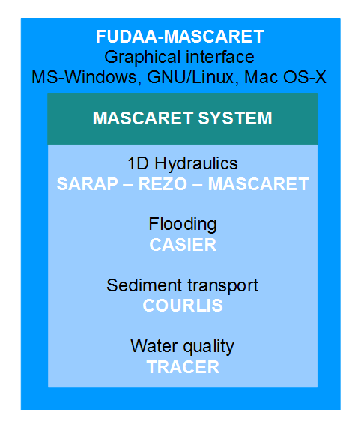
\includegraphics[scale=1.5]{Figures/MASCARET_system.eps}
  \caption{The \texttt{MASCARET} software}
 \end{center}
\end{figure}

The numerical methods used vary depending on whether the flows are steady or
unsteady, subcritical or supercritical and also depending on the type of
hydraulic network : branched network (subcritical steady flow engine) or meshed
network (subcritical unsteady flow engine). It is recalled that any branch
arrangement are allowed in a meshed network, whilst in a branched network there
is only one single path connecting two points of the network.

\subsection{General hypothesis}

The principal hypotheses justifying the modelling approach (1-D) used in the 3
hydraulic engines are stated below:

\vspace{0.5cm}
\begin{itemize}
 \item each reach has a prefered axis of flow, the velocity vectors are always
   considered parallel to this axis ;
 \item the flow has a small curvature in the horizontal plane ; the vertical
   accelerations are negligible, and the distribution of pressures is
   quasi-hydrostatic ;
 \item the average slope of the flow is small (the cosine of the angle between
   the horizontal and the bottom is close to 1) ;
 \item the viscosity shear stress on the bottom and the banks are taken into
   account using empirical friction laws (Strickler's relation).
\end{itemize}

\vspace{0.5cm}



Therefore, in each plane perpendicular to its axis, the flow is entirely determined by the values of the average velocity (or of the total flow), and of the elevation of the free surface.

\vspace{0.5cm}

A few other hypotheses are also considered in order to simplify the data entry process and consider only the most usual cases :
\vspace{0.5cm}
\begin{itemize}
 \item the influence of the wind is neglected;
 \item when a confluent is not modelled using a specific reach, it is assumed perpendicular to the main axis of flow: it is represented by a lateral flow input that does not add any momentum.
\end{itemize}

\vspace{0.5cm}

Other codes developed at EDF can be used when the hypotheses associated with \texttt{MASCARET} are too limiting, and complement the engines provided by \texttt{MASCARET}.
\vspace{0.5cm}
\begin{itemize}
 \item Two-dimensional flows can be treated with the \texttt{TELEMAC} system\cite{HERVOUET07};
 \item The geometry of the reaches is not evolving during the simulations. The \texttt{COURLIS} code, which uses the hydraulic engine of \texttt{MASCARET}, is dedicated to the treatment of solid transport and its consequences ;
 \item Extended inundation plains, where the flows is not one-dimensional, can be modelled with a system of inter-connected storage cells. The \texttt{CASIER} code can be linked to the unsteady subcritical flow engine to widens the field of application of the \texttt{MASCARET} system. It represents a network of reaches and associated storage cells (equivalent to quasi-2d modelling)
\end{itemize}

\subsection{Definitions and notations}

\subsubsection{Definitions} \label{secDef}

In the introduction we have outlined the basic characteristics of the modelling.  We consider subcritical and supercritical flows in networks of reaches, each reach having a principal axis of flow. The calculated values are always relative to a section of flow perpendicular to this axis, each section is identified by its abscissa along this axis.

\vspace{0.5cm}

The flow sections are considered to be the union of the three sub-sections:
%\vspace{0.5cm}
\begin{itemize}
 \item \underline{The low flow channel}, normal channel outside of flood periods. This channel can include islands but, if so, the elevation of the free surface is supposed to be identical on each side of the island. If this is not the case, one should resort to use a meshed network model ;
 \item \underline{The high flow channel}, additional sections of flow active in times of flood, when the water level rises above the crest of the right or left bank. These sections are represented on each side of the channel, the elevation of the two banks being generally distinct ;
 \item \underline{The storage zones}, treated like reservoirs, fill up as the flood rise and empty as water levels decrease. They act as water storage but, unlike the high flow channel, they do not convey any flow (the velocities in the direction of the axis of flow are supposed nil).
\end{itemize}

\vspace{0.5cm}

If the low flow channel is generally easy to identify, the limit between the high flow channel and storage zones is however much less well defined and can vary depending on the importance of the flood.

\vspace{0.5cm}

When the storage zones are likely to generate transverse flows in the floodplain, the present modeling approach becomes insufficient ; it is therefore necessary to couple \texttt{MASCARET} with a storage cell system.

\vspace{0.5cm}

It can be necessary to use a two-dimensional model instead of or in complement to the one-dimensional model, when the one-dimensional approach reaches its limits.

\vspace{0.5cm}

The estimation of the energy dissipated by friction is a fundamental element of the modelling. This is usually done with the Strickler roughness coefficient (see the following paragraph), it should be estimated separately in the low flow or high flow channel. The role of the calibration is to estimate the friction coefficients as well as possible by using the known natural level of the water. This calibration is often done by trial and errors. However, an optimisation algorithm has been specially developed for the steady flow engine, and this allows an automatic calibration of the friction coefficients.

Figure \ref{SchemProf} and its notations summarise the key elements of the modelling approach in a flow section.

\begin{figure}[h]
 \begin{center}
  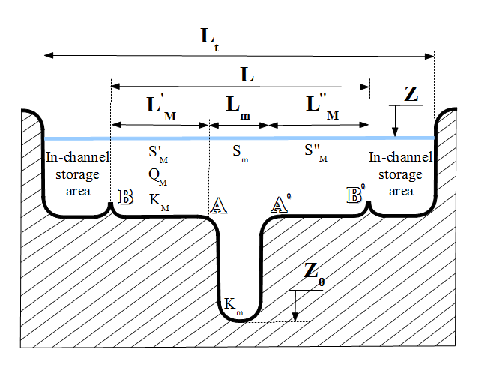
\includegraphics[scale=1.5]{Figures/Schema_profil.eps}
  \caption{Representation of a profile - Notations}
  \label{SchemProf}
 \end{center}
\end{figure}

\vspace{0.5cm}

\textbf{Comment :}
it is important to distinguish between the ``data'' sections (or profiles) where the geometry is calculated directly from topographic information (survey, digital terrain model), and the ``computation'' sections (chosen by the user) where the values will be obtained by interpolation between ``data'' profiles.
\textit{In the computational sections, the flow variables are interpolated between data sections, not the bathymetry/geometry}

\subsubsection{Notations} \label{secNot}

Unless otherwise stated, the following variables are used throughout the document (see figure \ref{SchemProf}) :
\vspace{0.5cm}
\begin{itemize}
 \item $t$ the time ($s$);
 \item $x$ the abscissa along the principal axis of flow in the river ($m$);
\vspace{0.5cm}
 \item $Q_m$ the discharge in the low flow channel ($m^3.s^{-1}$);
 \item $Q_M$ the discharge in the high flow channel, left and right bank ($m^3.s^{-1}$);
 \item $Q$ the total discharge in the active channel ($m^3.s^{-1}$) : $Q = Q_m + Q_M$;
 \item $q_l$ the lateral inflow contribution per meter length ($m^2.s^{-1}$);
\vspace{0.5cm}
 \item $L_m$ the surface width of the low flow channel ($m$);
 \item $L_M$ the surface width of the high flow channel ($m$) : $L_M = L^{'}_{M} + L^{''}_M$;
 \item $L$ the surface width of the active channel ($m$) : $L = L_m + L_M$;
 \item $L_s$ the width of the storage zones ($m$);
 \item $L_t$ the surface width of the total channel with storage ($m$);
\vspace{0.5cm}
 \item $S_m$ the area of the low flow channel or wetted cross section ($m^2$);
 \item $S_M$ the area of the high flow channel ($m^2$) : $S_M = S^{'}_{M} + S^{''}_M$;
 \item $S$ the area of the active bed ($m^2$) : $S = S_m + S_M$;
 \item $S_s$ the area of the active channel ($m^2$);
 \item $S_t$ the area of the total channel with storage ($m^2$);
\vspace{0.5cm}
 \item $K_m$ the Strickler coefficient of the low flow channel;
 \item $K_M$ the Strickler coefficient of the high flow channel;
\vspace{0.5cm}
 \item $P_m$ the wetted perimeter of the low flow channel ($m$) : $P_m = AA^{'}$;
 \item $P_M$ the wetted perimeter of the high flow channel ($m$) : $P_M = A^{'}B^{'}+AB$;
 \item $P$ the wetted perimeter of the active channel ($m$) : $P = P_m + P_M$;
\vspace{0.5cm}
 \item $R_m$ the hydraulic radius of the low flow channel ($m$) : $R_m = S_m / P_m$;
 \item $R_M$ the hydraulic radius of the high flow channel ($m$) : $R_M = S_M / P_M$;
 \item $R$ the hydraulic radius of the active channel ($m$) : $R = S / P$;
\vspace{0.5cm}
 \item $V_m$ the velocity of water in the low flow channel ($m.s^{-1}$) : $V_m = Q_m / S_m$;
 \item $V_M$ the velocity of water in the high flow channel ($m.s^{-1}$) : $V_M = Q_M / S_M$;
 \item $V$ the mean velocity of the flow ($m.s^{-1}$) : $V = Q / S$;
\end{itemize}

\vspace{0.5cm}
